\documentclass[11pt]{article}

\usepackage{graphicx}
\usepackage[utf8]{inputenc}
\usepackage{hyperref}
\usepackage{mathtools}
\usepackage{float}
\usepackage[margin=0.5in]{geometry}

\begin{document}
\setlength{\textwidth}{20cm}
\setlength{\textheight}{22cm}
\title{\Huge\textbf{Neural Networks}\linebreak \small{Predicting student performance} \linebreak\linebreak
\Large\textbf{Intermediate Report}\linebreak\linebreak
\linebreak\linebreak

\includegraphics[scale=0.1]{feup-logo.png}\linebreak\linebreak
\linebreak\linebreak
\Large{Mestrado Integrado em Engenharia Informática e Computação} \linebreak\linebreak
\Large{Inteligência Artificial}\linebreak\linebreak
\Large{Group E5\_1}
}

\author{
Gonçalo Lopes\\ up201303198\\
\and
Ivo Fernandes\\ up201303199\\
}
\date{\today}
\maketitle
\newpage
\tableofcontents
\newpage

\section{Objective}

The purpose of this project is to train an Artificial Neural Network, using the Back-Propagation algorithm, in order to predict student performance based on attributes for each student, taking into account aspects of the student's private and work life and also attributes like their gender and age.

\section{Description}
\subsection{Specification}

\subsubsection{Project phases}
\label{sec:phases}
To complete this project the group will have to:
\begin{enumerate}
\item Understand the structure of a neural network
\item Understand the mechanism of the back-propagation algorithm
\item Choose a back-propagation framework and learn it
\item Learn how to train neural networks
\item Build different networks and train them
\item Compare the networks, try different training methods, handle the data-set
\item Construct a final network and evaluate its accuracy
\end{enumerate}

\subsubsection{Network Structure}
\label{sec:network}
A neural network is comprised of 3 types of layers, each layer containing nodes that represent neurons.
\begin{itemize}
\item Input Layer
\item Hidden Layers
\item Output Layer
\end{itemize}

Each layer can have a different number of nodes and all of a layer's nodes are connected to all of the next layer's nodes. There is only one input layer and one output layer. There can be any number of hidden layers, each with any number of nodes. To solve most problems, only one hidden layer is required. Usually, the output layer consists of a single node. 
A neuron consists of 5 main parts:
\begin{enumerate}
\item The \textbf{input}, through which the neuron receives information
\item The \textbf{connection weights}, that determine how much influence each input value has
\item The \textbf{combination function}, which is usually a sum of the input values times their respective weights
\item The \textbf{activation function}, which calculates the state of the neuron. The function used is usually the sigmoid function $\frac{1}{1+e^{-\alpha}}$ This function is used because it introduces non-linearity in the network, as opposed to using a step function. This function is also continuous and differentiable. Take $\beta = \frac{1}{1+e^{-\alpha}}$, $\frac{\partial\beta}{\partial\alpha}$ = $\beta (1-\beta)$
\item The \textbf{output}, which is the result of the transfer function. If we didn't introduce non-linearity by using the sigmoid function, output $s_i \in \{0, 1\}$. Since we introduced non-linearity, output $s_i \in [0, 1]$.
\end{enumerate}
\begin{figure}[H]
\label{fig:example}
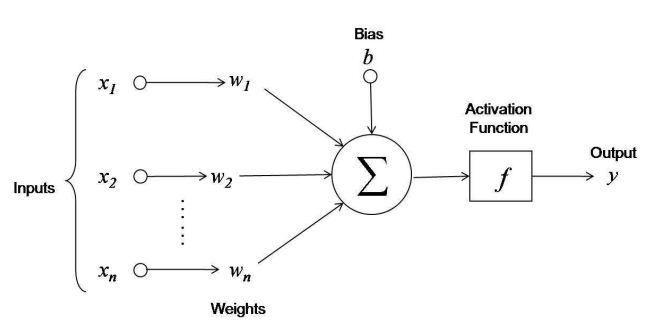
\includegraphics[scale=0.5]{neuron.jpg}
\centering
\caption{Example of a neuron, taken from \url{https://blogs.cornell.edu/info2040/2015/09/08/neural-networks-and-machine-learning/}}
\end{figure}
\hfill \break
\hfill \break

\subsubsection{Back-propagation Algorithm}
\label{sec:back}
Let $\overrightarrow{z}$ = $f(\overrightarrow{x}, \overrightarrow{w}), \overrightarrow{z}$representing the output of the neural network for the set of inputs $\overrightarrow{x}$ and set of weights $\overrightarrow{w}$
Let $\overrightarrow{d}$ = $g(\overrightarrow{x}), \overrightarrow{d}$ representing the desired output of the neural network for the set of inputs $\overrightarrow{x}$
To calculate how well the network is doing we must calculate a function that includes the difference between $\overrightarrow{d}$ and $\overrightarrow{z}$. 
Let P($\overrightarrow{d}, \overrightarrow{z}$) = $\frac{1}{2} || \overrightarrow{d} -  \overrightarrow{z} ||$, we will call this the Performance function.
\hfill \break
\hfill \break
We want to minimize the Performance function, minimizing it means minimizing the difference between the desired output and the real output, which means this is the direction to go, to make the network learn.

For explaining the back-propagation algorithm we will always refer to a simple network with 1 input node and 1 hidden node.
For a network with 2 nodes, 2 weights, w1 and w2, $\Delta w = r(\frac{\partial P}{\partial w_1} , \frac{\partial P}{\partial w_2})$, r is the \textbf{learning rate}. As the name suggests, the learning rate will help the network learn faster, however, this rate cannot be too high. If the learning rate is too high, while trying to fit to the curve of the desired weights, the algorithm will get into a feedback loop, never converging to the minimum and learning nothing.
\begin{figure}[H]
\label{fig:example}
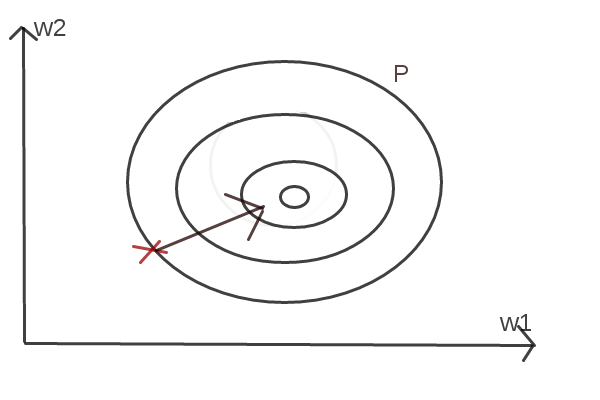
\includegraphics[scale=0.3]{performance.png}
\centering
\caption{For 2 weights, w1 and w2, we are trying to move in the direction that minimizes the P function}
\end{figure}
Since we picked the sigmoid function for our activation function, calculating $\Delta \overrightarrow{w}$ becomes simple.
Let:
\begin{itemize}
\item x be the input of node 1
\item y be the output of node 1, input of node 2
\item z be the output of node 2, the output of the network
\end{itemize}

$\frac{\partial P}{\partial w_2} = (d-z)z(1-z)y$

$\frac{\partial P}{\partial w_1} = (d-z)z(1-z)yw_2x(1-y)$

But we already calculated $(d-z)z(1-z)y$, which is $\frac{\partial P}{\partial w_2}$

This means that a given node's weight depends on the node's input, output, the weight of the next node and the partial derivative of the next node.
This gives the back-propagation algorithm its name. We propagate the error, $\frac{\partial P}{\partial w_2}$, backwards, in order to calculate $\Delta \overrightarrow{w}$, the vector containing the error for each weight.

By using multiple iterations, the algorithm adjusts the weights of the network, minimizing the performance function.

\begin{figure}[H]
\label{fig:example}
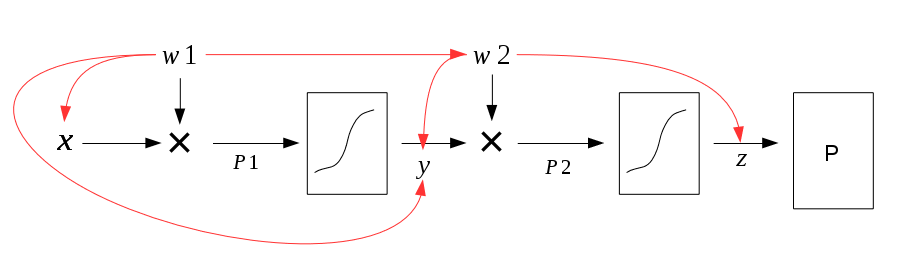
\includegraphics[scale=0.4]{example.png}
\centering
\caption{Example network with 1 input node and 1 hidden node, red arrows represent dependence.}
\end{figure}

The calculation of $\Delta \overrightarrow{w}$ may also be influenced by \textbf{momentum}. To incorporate momentum into the calculation, the new formula is:

$\Delta \overrightarrow{w}(t) = r(\frac{\partial P}{\partial w_1} , \frac{\partial P}{\partial w_2}) + m \Delta \overrightarrow{w}(t-1)$, t is the iteration number, m the momentum constant. The momentum is usually set to a high value between 0 and 1.

When we calculate $\Delta w$ we are going along the gradient of the activation function, in the direction specified by the output error. If by going along this direction, we skip the ideal point for the weights, we must go back. Momentum helps with this situation, if the algorithm was moving in a direction and it suddenly changes directions, the first step will be small, since it takes into account the direction of the last step, which was opposite to the direction of the new step.
\hfill \break
\hfill \break
A factor that may lead to unsuccessfully training the network is the number of iterations. If the number of iterations is too high overfitting may start to happen. Over fitting is when the algorithm tries so hard to fit to the sample (training set) that values nearby the ones used may become distorted, and when faced with a similar situation the network will output a very different value.
\hfill \break
\hfill \break
The back-propagation algorithm must also shuffle the dataset instances before starting each iteration, otherwise it will be unable to successfully train. The chosen framework does this.
\subsubsection{Training a series of Networks for the same dataset}
\label{sec:training}
The data-set to be used on the project has \href{http://archive.ics.uci.edu/ml/datasets/Student+Performance}{\underline{33 attributes and 649 instances}}. 
The 33rd attribute of the data-set is the final grade, this will be our single output node. This means that, initially, there will be 32 input nodes.
One of the main purposes of the project, is treating the dataset, reducing non-important attributes. This will make the network training more efficient, since there will be less nodes to weight.

The framework we will be using restricts the inputs and outputs to be in the range [0, 1], so to train and test our network we need to first parse the data and transform all the inputs into the corresponding value in the range [0, 1].
\hfill \break
\hfill \break
To train and test the network we will have to divide the dataset into two separate groups. The \textbf{Training Set} and the \textbf{Test Set}, these groups will be used to train different networks, however, they will be the same for all the networks. We could use a \textbf{Validation Set}, but since we only have 649 instances, having 3 disjoint sets would mean small sets, thus, we chose not to use the Validation Set, which may or may not be used in the training of a neural network.

We will keep the Training Set size at 2/3 of the number of instances and the Test Set at 1/3, as it is usual to follow this approach. 
\hfill \break
\hfill \break
As described in the \hyperref[sec:network]{Network} section, the network may have any number of hidden layers, each with any number of nodes. We must fiddle with these values while creating different networks, in order to create better networks with faster training times and better accuracy.
\hfill \break
\hfill \break
The network's learn rate and momentum may also be adjusted. We already discussed where these attributes affect the algorithm in the \hyperref[sec:back]{previous} section.
\hfill \break
\hfill \break
We can also adjust the error threshold to be achieved, which means that when the back-propagation calculated error is below the threshold, the training of the network stops.
\subsection{Expected Results and Tests}
From training different networks, and fiddling with the attributes referenced in the \hyperref[sec:training]{training} section, we expect to see different training times and network accuracies. 

We are unable to set an accuracy goal for our final network, but we hope to see a noticeable increase when comparing our final network to our first.

\newpage
\section{Development}
The project is being developed on Debian "Jessie".

We are using \href{https://github.com/harthur/brain}{\textbf{BrainJS}}, as our neural network framework.

Since we are using a Javascript framework, we decided to create a web interface, using HTML, CSS and Javascript, that allows us to change training options, create, save and load data sets  and train networks, automatically calculating:

\begin{itemize}
\item Number of iterations
\item Error threshold achieved in training
\item Training time
\item Pass course accuracy
\item Final grade accuracy
\end{itemize}

\textbf{Pass course accuracy} is defined by the network's ability to predict if a student will pass or fail the course. While testing, the network compares to expected grade to the predicted grade, after rounding the predicted grade. If both grades are greater or equal to 10, or both are lower than 10, it's a \textbf{yes} for the \textbf{Pass course accuracy}, otherwhise, it's a \textbf{no}.

\textbf{Final grade accuracy} is defined by the network's ability to predict a student's final grade. While testing, the network compares to expected grade to the predicted grade, after rounding the predicted grade. If both grades are equal, then it's a \textbf{yes} for the \textbf{Final grade accuracy}, otherwhise, it's a \textbf{no}.
\hfill \break
\hfill \break
The implementation allows us to feed in a data-set, which creates the Training and Test Set according to the inputed sizes. 

For this project we will be analysing two different data sets, the portuguese and math sets. Since the students in each data set are different, the sets must be handled separately. We will only create one training and test set for each data set, in order to use the same sets for all the experiments. The Training Sets are 70\% of the data set and the Test Sets the remaining 30\%. 

On the created web interface, we are also allowed to manipulate the number of hidden layers and hidden nodes, and input and output nodes. This way we can easily remove some nodes from the neural network and perform experiments.

\section{Experiments}
In this section, we will perform all the experiments and discuss the results.

The objective of the experiments is to identify the optimal neural net structure and identify which inputs really affect the output. This is done so that the neural network trains in the least amount of time and the training results are the best possible with the current data set available.

When specifying the number of hidden layers and hidden nodes used, the following representation is used:
\textit{\{nodes\_First\_layer, nodes\_Second\_layer, ...., nodes\_N\_layer\}}

The removed column on the tables specifies the input nodes that were removed for that execution.

Since the used framework is based on Javascript, training times will be higher than if a Java or C++ framework was used. However, iteration growth will be the same. We will only present the number of iterations for each train+test, not specifying the time. The time may also vary from what other work the browser is doing, which means it would not be a meaningful metric.

The training and test sets are obtained only once for each data-set. These sets are obtained after shuffling the data-set, in order to achieve plausible results. If the data-set was not shuffled, the train set might contain very similar instances, and all of them very different from the instances on the test set, which would lead to bad accuracy. 

Since the data-set is only shuffled once to create the training and test set. Maybe the resulting shuffle is a bad one, this means that all following experiments will have either all higher or all lower results on experiments, however, the difference between experiments will still be noticeable. Nonetheless, this wouldn't happen if the original data-set was large and representative enough. Which does not happen because the data-sets have less than 400 instances, for what is a complicated problem.

The training set is also shuffled between each training iteration.

\subsection{The quitters}
A quitter is a student who either failed the course due to too many absences, or decided to drop out. This means the quitter will have a G3 of 0. 

We will use the Math dataset for this experiment, the same result is expected from the Portuguese dataset.

Using the \textbf{default data-set:} 

\begin{tabular}{| c | c | c | c | c | c | c | c |}
\hline \textbf{min\_thresh} & \textbf{hidden} & \textbf{learn\_rate} & \textbf{momentum} & \textbf{removed} & \textbf{iterations} & \textbf{PassAcc} & \textbf{GradeAcc}\\
\hline 0.005 & \{1\} & 0.3 & 0.8 & \_ & 260 & 90\% & 64\%\\
\hline 0.0005 & \{1\} & 0.3 & 0.8 & \_ & 1693 & 80\% & 41\%\\
\hline 0.0005 & \{1\} & 0.2 & 0.9 & \_ & 2380 & 81\% & 49\%\\
\hline 0.0005 & \{5\} & 0.2 & 0.9 & \_ & 2519 & 82\% & 46\%\\
\hline 0.0005 & \{10,5\} & 0.2 & 0.9 & \_ & 2457 & 81\% & 40\%\\
\hline
\end{tabular}

\hfill \break
\hfill \break
Using the \textbf{no-quitters data-set:} 

\begin{tabular}{| c | c | c | c | c | c | c | c |}
\hline \textbf{min\_thresh} & \textbf{hidden} & \textbf{learn\_rate} & \textbf{momentum} & \textbf{removed} & \textbf{iterations} & \textbf{PassAcc} & \textbf{GradeAcc}\\
\hline 0.005 & \{1\} & 0.3 & 0.8 & \_ & 19 & 91\% & 70\%\\
\hline 0.0005 & \{1\} & 0.3 & 0.8 & \_ & 1666 & 89\% & 64\%\\
\hline 0.0005 & \{1\} & 0.2 & 0.9 & \_ & 1987 & 86\% & 59\%\\
\hline 0.0005 & \{5\} & 0.2 & 0.9 & \_ & 2218 & 92\% & 63\%\\
\hline 0.0005 & \{10,5\} & 0.2 & 0.9 & \_ & 2057 & 93\% & 62\%\\
\hline
\end{tabular}

\hfill \break
\hfill \break

For the default set, with the default min threshold, the pass accuracy is the same as for the no-quitters set. After lowering the min threshold 10 times, the pass accuracy stays the same for the no-quitters set but drops almost 10\% on all the following experiments for the default set. As for the grade accuracy, it drops an average of 7\% for the no-quitters set and an average of 20\% for the default set. This is due to overfitting, and this is why the experiments included lowering the learning rate and momentum and changing hidden layers. However, the obtained results were not much different.
\hfill \break
\hfill \break
\textit{Why do both sets suffer from overfitting?} 

This happens because, as already referenced, the datasets are small and not very representative. 

\newpage
\textit{Why does grade accuracy drop more on the default set than pass accuracy, when compared to the value changes for the no-quitters set?}

Because when a student has a 0, and the network calculates for example a 5 for that student, even though the grade error is large, the pass result is still the same. 

\begin{figure}[H]
\label{fig:Pass vs Grade}
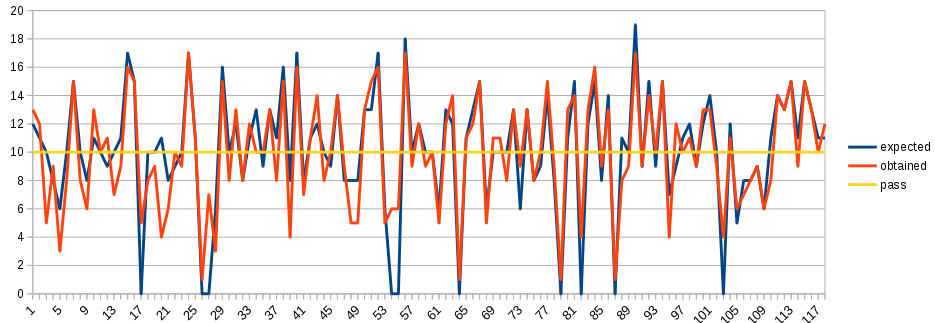
\includegraphics[scale=0.6]{passgrade.png}
\centering
\caption{Pass vs Grade accuracy (default)}
\end{figure}

The pass accuracy only fails when the expected and obtained values are on different sides of the pass line. This did not happen for any of the quitters. 

\begin{figure}[H]
\label{fig:Pass vs Grade}
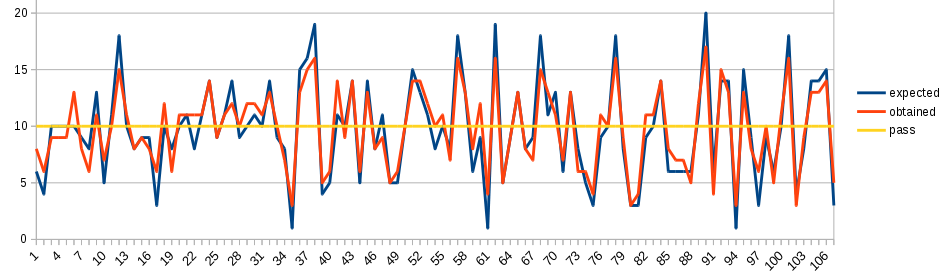
\includegraphics[scale=0.6]{passgradenoquit.png}
\centering
\caption{Pass vs Grade accuracy (no-quitters)}
\end{figure}

\textit{Why does the default set have worse results than the no-quitters set?}

Because there is more overfitting on the default set, due to quitters. A quitter might have the same input values as someone who passed the course, but because of quitting, the result is 0. This leads to the network giving lower grades to students that did not quit.

When comparing both graphs, we can clearly see the default network overfitting students and giving them a lower grade, while also giving quitters a higher grade than 0.

\hfill \break
\hfill \break

We can also observe on the 2 graphs that, due to data-set shuffling, the default test set had no students with G3 of 20, while the no-quitters set had a student with a G3 of 20. Having a 20 on the test set will reduce grady accuracy because it is hard to predict a 20, since it is the highest value possible. We can see on the graphs that high expected grades have lower obtained values and low expected grades have higher obtained values. The obtained values tend towards the mean. 

\hfill \break
\hfill \break
\textbf{Conclusion:}

The following experiments will all be done on the no-quitters data-set.

\subsection{G1 and G2}
We expect G1 and G2 to be have a very strong influence on the result of G3, so we will test that.
\hfill \break
\hfill \break
\begin{tabular}{| c | c | c | c | c | c | c | c |}
\hline \textbf{min\_thresh} & \textbf{hidden} & \textbf{learn\_rate} & \textbf{momentum} & \textbf{removed} & \textbf{iterations} & \textbf{PassAcc} & \textbf{GradeAcc}\\
\hline 0.005 & \{1\} & 0.3 & 0.8 & \_ & 19 & 91\% & 70\%\\
\hline 0.005 & \{1\} & 0.3 & 0.8 & \_G1\_G2\_ & 467 & 59\% & 24\%\\
\hline 0.005 & \{1\} & 0.3 & 0.8 & \_G2\_ & 276 & 90\% & 45\%\\
\hline 0.005 & \{1\} & 0.3 & 0.8 & \_G1\_ & 21 & 89\% & 70\%\\
\hline
\end{tabular}

When removing both G1 and G2, pass accuracy drops 1/3 and the grade accuracy drops 2/3. As expected, the grade accuracy always drops more than the pass accuracy.
\hfill \break
\hfill \break
When removing either G1 or G2, the pass accuracy stays more or less the same. This happens because knowing a student's grades on G1 or G2 has a high impact on predicting if the student will pass or not. 
\hfill \break
\hfill \break
When removing G1, the grade accuracy is almost half of when removing G2. This is because the G2 grade is a lot closer to the G3 grade than the G1. The value of G2 is depends on the value of G1, so, having G2 and not having G1 means that G1 still has some effect on the result.

We chose to perform our following experiments without G1 or G2 on our input nodes. We found it to be more interesting to detect how high can the accuracy of the network go without these input nodes, as predicting a student's grades while having the grades as input doesn't sound like predicting at all.

The following experiments will be done separately for the Math students data set and for the Portuguese students data set, as the data is from different students, we are unable to join the data and have a network with 2 outputs, which would be one for Math G3 and another for Portuguese G3.

\subsection{Math}
\subsubsection{Default network}
\subsubsection{Meaningless inputs}
First, we will try to find inputs that can be removed from the network that are making the network slower, perhaps making it suffer from over fitting and not contributing to accuracy. The first input nodes to be evaluated are ones that one can guess will be meaningless.
\subsubsection{The schools}
After a quick look at the data sets, we can see that there are only 2 schools, \textit{Gabriel Pereira} and \textit{Mousinho da Silveira}. Seeing as only 2 schools are in the data set, if both schools' students have similar average grades, the network output will be the same, or better. 

\begin{tabular}{| c | c | c | c | c | c | c | c |}
\hline \textbf{min\_thresh} & \textbf{hidden} & \textbf{learn\_rate} & \textbf{momentum} & \textbf{removed} & \textbf{iterations} & \textbf{PassAcc} & \textbf{GradeAcc}\\
\hline 0.005 & \{1\} & 0.3 & 0.8 & \_G1\_G2\_ & 463 & 60\% & 26\%\\
\hline 0.005 & \{1\} & 0.3 & 0.8 & \_school\_G1\_G2\_ & 549 & 55\% & 22\%\\
\hline
\end{tabular}

After removing the school input, the network's accuracy dropped. After this we have a hint that the schools' average grades differ. 

The calculated average grades are:
\hfill \break
\hfill \break
\begin{tabular}{| c | c |}
\hline \textbf{School} & \textbf{Average Grades}\\
\hline MS & 10.79\\
\hline GP & 11.62\\
\hline
\end{tabular}

As was expected from our observation of the changes on the network's accuracy, the school's average grades are differ in almost 1 value.
\subsubsection{Deprecated Inputs}
\paragraph{Experiments}
\paragraph{Results}
\subsubsection{Parameter Values}
\paragraph{Experiments}
\paragraph{Results}



\subsection{Portuguese}
\subsubsection{Neural Net Structure}
\paragraph{Experiments}
\paragraph{Results}
\subsubsection{Deprecated Inputs}
\paragraph{Experiments}
\paragraph{Results}
\subsubsection{Parameter Values}
\paragraph{Experiments}
\paragraph{Results}
\section{Conclusions}
So far we have learned how a neural network is structured, how the back-propagation algorithm works and how to differently train networks in order to achieve different results.

Learning this subject was fun because of how easy it is to be impressed by machines learning through training. And now we have some knowledge of how it works.
\section{Improvments}

\section{Resources}

\subsection{Bibliography}

\url{https://web.fe.up.pt/~eol/IA/1516/APONTAMENTOS/7_RN.pdf}

\href{https://www.youtube.com/watch?v=q0pm3BrIUFo}{Neural Nets, Back Propagation, Patrick Winston, M.I.T.}

\url{http://www.faqs.org/faqs/ai-faq/neural-nets/}

\url{http://stats.stackexchange.com/questions/181/how-to-choose-the-number-of-hidden-layers-and-nodes-in-a-feedforward-neural-netw}

\url{http://www.akamaiuniversity.us/PJST9_1_72}

\url{https://takinginitiative.wordpress.com/2008/04/23/basic-neural-network-tutorial-c-implementation-and-source-code/}

\url{https://github.com/harthur/brain}

\subsection{Software}

To train the network, we will use the javascript framework \href{https://github.com/harthur/brain}{\textbf{BrainJS}}, an open source implementation of a neural network, using the back-propagation algorithm, implemented using the basic sigmoid function.

\newpage
\section{Appendix}
In this section we present the different interface menus.

\begin{figure}[H]
\label{fig:example}

\includegraphics[scale=0.3]{interface0.png}
\centering
\caption{User can either create network from data set or load existing network.}
\end{figure}

\begin{figure}[H]
\label{fig:example}
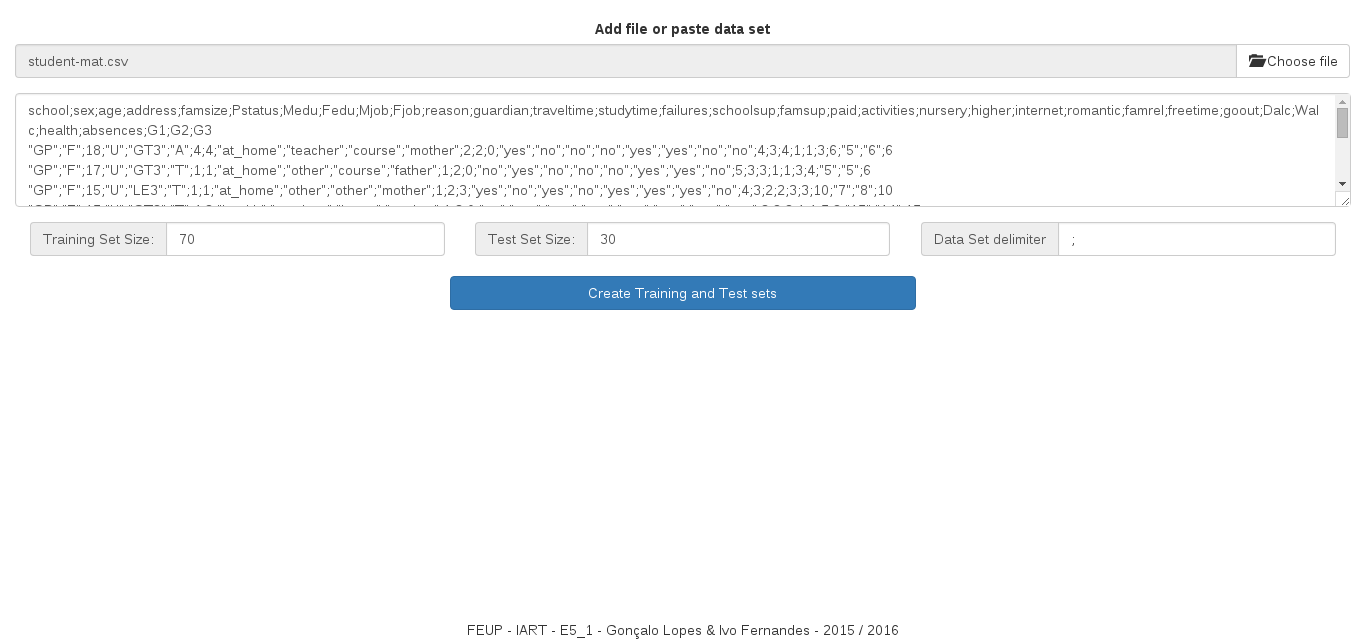
\includegraphics[scale=0.3]{interface1.png}
\centering
\caption{Create network interface.}
\end{figure}

\begin{figure}[H]
\label{fig:example}
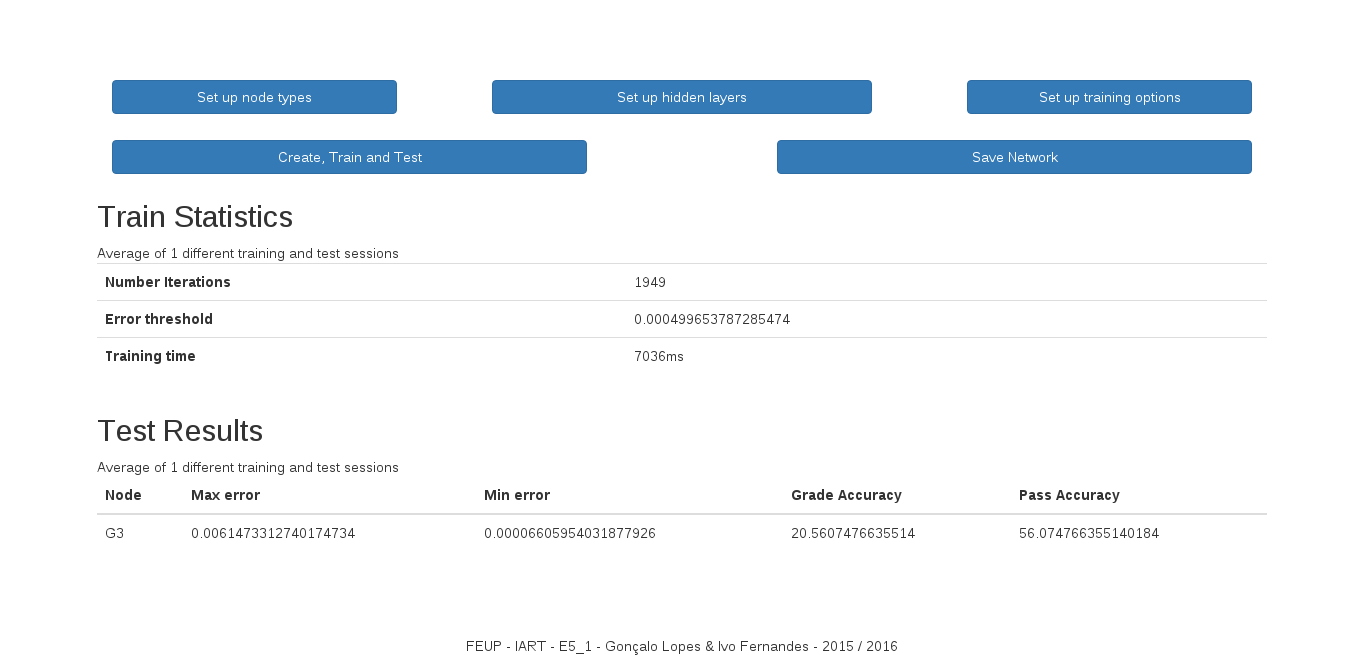
\includegraphics[scale=0.3]{interface2.png}
\centering
\caption{Train and test results and training options.}
\end{figure}

\begin{figure}[H]
\label{fig:example}
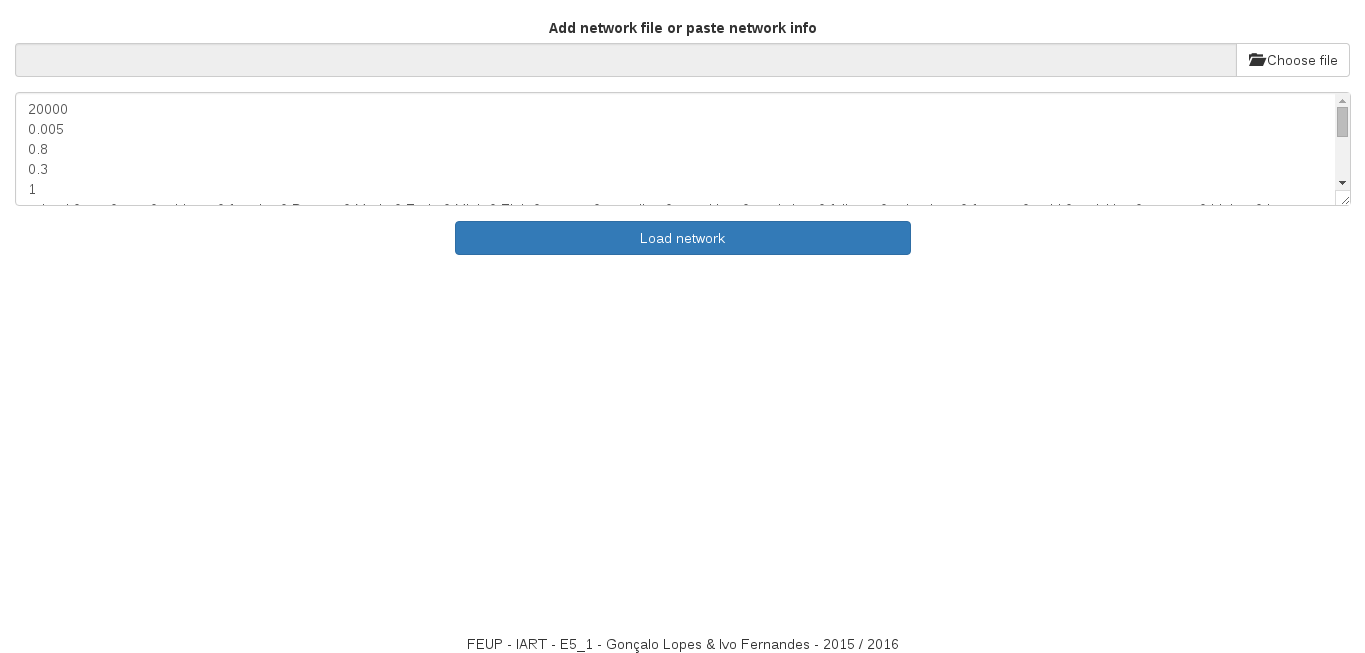
\includegraphics[scale=0.3]{interface3.png}
\centering
\caption{Load network interface.}
\end{figure}
\end{document}